% File: main.tex
% Date: 2015, April
% Authors: Gustavo Peixoto, Leon Lima.
% Description: Latex template file for seminar short papers presented at PPG-EM/UERJ.
% Version: 1.0
% Available online on: www.gesar.uerj.br

%% PREAMBLE
\documentclass[date,twocolumn,a4paper]{ppgem} 
\usepackage{amsmath}
\usepackage{enumitem}
\usepackage{pgfplots}
\usepackage{tikz}
\usepackage{pgf-pie}
\usepackage{minted}
\usepackage{float}
\usepackage{graphicx} % Required for \includegraphics
\usepackage[numbers, sort&compress]{natbib}  % citações numéricas por padrão
% \usepackage{biblatex}



\setlist{nolistsep}


%% TITLE
\Title{
Python: Paradigma Funcional Aplicado à Transformação de Dados
}

% PLEASE, DO NOT CHANGE THE PAGENUMBER{2}
\PageNumber{2}

% %% INSTITUTION
% \InstA{Rio de Janeiro State University} 
% \InstB{} 

\pagestyle{fancy}


\newenvironment{pythoncode}[1][]{%
    \minted[%
        linenos,
        xleftmargin=2mm,
        tabsize=2,
        breaklines,
        autogobble,
        numbersep=5pt,
        #1 % Allow optional extra parameters
    ]{python}%
}{%
    \endminted%
}

\begin{document}
    \thispagestyle{plain}
    \makeheader

    % Define a new float type for "Figura" with its own counter
    \newfloat{figlisting}{htbp}{lof}%[chapter] % [chapter] resets counter per chapter (optional)
    \floatname{figlisting}{Figura} % Sets the caption name
    \newcommand{\listoffiguras}{\listof{figlisting}{Lista de Figuras}} % Optional: Create a list of figuras

    % Keep the original "listing" environment for "Código"
    \floatname{listing}{Código} % Ensure the original listing uses "Código"
    \newcommand{\listofcodigos}{\lstlistoflistings} % Optional: List of code listings

    %% KEYWORDS
    % \begin{keywords}
    % Max of 4 keywords, comma separeted, {\LaTeX} typesetting, standardization.
    % \end{keywords}

    %% BODY
    \section*{RESUMO}
    Resumo aqui

    \section{INTRODUÇÃO}


    \section{OBJETIVO}
    O objetivo deste estudo é escrever código manutenível e de fácil compreensão se utilizando da abordagem funcional
    afim de demonstrar os efeitos positivos da mesma.

    
\section{METODOLOGIA}
% O objetivo desta pesquisa é escrever código mantenível e de fácil compreensão, a fim de demonstrar os efeitos positivos do paradigma funcional. Para isso, serão comparadas (através de exemplos práticos) as abordagens de resolução de problemas sob as perspectivas do paradigma não funcional e funcional. Essa comparação permitirá avaliar as diferenças entre os paradigmas e observar características como:

% * Facilidade de compreensão
% * Facilidade de manutenção
% * Clareza do código
% * Entre outros aspectos relevantes
Este estudo adotará uma abordagem comparativa entre os paradigmas funcional e imperativo, analisando soluções para problemas comuns em ambas as abordagens. A metodologia consistirá em:
\begin{enumerate}
    \item Seleção de Problemas: Escolha de um problema representativo, computacionalmente resolvível.
    \item Implementação Comparada: Desenvolvimento das soluções em na abordagem funcional e imperativa
    \item Análise Quantitativa: Avaliação de aspectos como:
    \begin{enumerate}
        \item Quantidade de linhas de código
        % \item Tempo de execução
        % \item Uso de métricas como complexidade ciclomática e linhas de código (LOC) para apoio quantitativo.
    \end{enumerate}
    \item Análise Qualitativa: Avaliação de aspectos como:
    \begin{enumerate}
        \item Facilidade de compreensão
        \item Legibilidade (mediante revisão por pares)
        \item Manutenibilidade (tempo para introduzir modificações)
        \item Clareza (análise de estrutura e redundância)
    \end{enumerate}
    \item Ferramentas: Todo o trabalho será desenvolvido utilizando a linguagem python
        e o ambiente de \textit{notebooks} do \textit{jupyter}\footnote{
             Ambiente web interativo para criar documentos com código, texto (Markdown), fórmulas e gráficos. Usa formato JSON (.ipynb) organizado em células de entrada/saída\cite{wiki_jupyter_notebook}.
        }
\end{enumerate}

    \section{FUNDAMENTOS TEÓRICOS}
O Paradigma de Programação Funcional (abreviado do inglês como \textbf{FP}, \textit{\textbf{Functional Programming}}), é um modo de pensar
a resolução dos problemas computáveis a partir da composição de funções\cite{queiroz_func_prog}.\\
Linguagens que oferecem total suporte a este paradigma geralmente permitem que funcções sejam atribuídas a variáveis, passadas como parâmetros
e retornadas de outras funções.
\subsection{Funções puras}
Pode-se dizer que uma função é pura quando retorna sempre a mesma saída, dados os mesmos argumentos\cite{queiroz_func_prog}. Em resumo, as funções
puras não podem alterar nenhum estado externo ao seu escopo\footnote{Contexto onde variáveis/expressões são acessíveis. Escopos filhos herdam dos pais, mas não o contrário. Funções criam escopos isolados (ex.: variáveis internas não são acessíveis externamente)\cite{mdn_escopo}.}.\\
\textbf{Exemplo:}
Digamos que queira-se implementar um contador para uso geral conforme código abaixo. Os incrementos de valores sempre são dados através da função
\textbf{incrementa} definida na linha 3.
\begin{listing}[!ht]
    \begin{minted}[linenos,xleftmargin=2mm,tabsize=2,breaklines,autogobble,numbersep=5pt]{python}
        contador = 0

        def incrementa(valor):
            contador += valor
            return contador

        print(incrementa(5))
        # Saída: 5 (esperado)
        print(incrementa(2))
        # Saída: 8 (esperado)
    \end{minted}
    \caption{Exemplo de função impura}
    \label{listing:impura}
\end{listing}
\\Observa-se nas linhas 7 e 9 que as chamadas à função \textbf{incrementa} retorna os resultados esperados.\\
Agora, digamos que em algum ponto do programa a variável \textbf{contador} seja alterada conforme o
Código \ref{listing:impura-retorno}:

\begin{listing}[!ht]
    \begin{minted}[linenos,xleftmargin=2mm,tabsize=2,breaklines,autogobble,numbersep=5pt,firstnumber=12]{python}
        contador = 100
        print(incrementa(5))
        # Saída: 105 (inesperado)
    \end{minted}
    \caption{Retorno inesperado de função impura}
    \label{listing:impura-retorno}
\end{listing}\pagebreak

Percebe-se na saída da linha 13, que a chamada da função \textbf{incrementa} com parâmetro 5 retorna resultados imprevisíveis. Ao comparar
a linha 13 com a linha 7 do Código \ref{listing:impura}, nota-se claramente a quebra do conceito de função pura. Isto introduz comportamentos inconssistentes
que podem levar a \textit{bugs}\footnote{
    Erro em sistemas eletrônicos/software que causa comportamentos inesperados (ex.: travamentos, resultados incorretos). Pode surgir no código-fonte, frameworks, SO ou compiladores. Comum em computação, jogos e cibernética\cite{wiki_bug}.
} inesperados no código. Bugs desta natureza geralmente são difíceis de rastrear, a situação é ainda
mais sensível em códigos de natureza \textit{\textbf{Multi-Threading}}\footnote{
    Paradigma que aumenta a eficiência do sistema ao executar múltiplas threads/tarefas simultaneamente, assim como o multiprocessamento. Essencial para a computação moderna\cite{wiki_multithreading} (adaptado).
}.\\
Em resumo: Qualquer função que altere estados fora de seu escopo é impura por natureza, pois a alteração de estados globais geram escopos compartilhados em que um mesmo recurso pode ser concorrentemente disputado.
É este tipo de abordagem que leva a problemas de deadlock\footnote{
    Impasse em que processos ficam bloqueados mutuamente, cada um esperando por um recurso retido por outro. Comum em SOs e bancos de dados, ocorre mesmo com recursos não-preemptíveis (ex.: dispositivos, memória), independente da quantidade disponível. Pode envolver threads em um único processo\cite{wiki_deadlock}.
} e os mais derivados problemas em computação concorrente e parelela. Desta forma o uso de semáforos, filas e etc acabam sendo obrigatórios, adicionando grandes complexidades ao código fonte.

\subsubsection{Purificando a função}
O Código \ref{listing:purificada} demonstra a versão purificada da função \textbf{incrementa} na linha 3:
\begin{listing}[!ht]
\begin{minted}[linenos,xleftmargin=2mm,tabsize=2,breaklines,autogobble,numbersep=5pt]{python}
    contador = 0

    def incrementa(original, valor):
        return original + valor


    print(contador:=incrementa(contador, 5))
    # Saída: 5 (esperado)
    print(contador:=incrementa(contador, 2))
    # Saída: 8 (esperado)

    contador = 100
    print(contador:=incrementa(contador, 5))
    # Saída: 105 (esperado)
\end{minted}
\caption{Função purificada}
\label{listing:purificada}
\end{listing}\linebreak

Nota-se que as saídas nas linhas 7, 9 e 13 são as mesmas da versão anterior do código. A diferença é que agora a função
\textbf{incrementa} não altera nenhuma variável/estado externo ao seu escopo. Sempre que \textbf{incrementa} é chamada,
a variável \textbf{contador} é atualizada com o novo valor do retorno da função. Observa-se agora que na linha 13 a saída
105 é esperada, pois o parâmetro não depente mais somente do valor 5 a ser incrementado, mas também do valor original de
\textbf{contador}.
Desta forma, a função torna-se pura por não alterar escopos externos a ela. De certa forma, pode-se dizer que a função está a trabalhar
com o conceito de \textbf{imutabilidade} dentro dos limites de seu escopo (embora \textbf{contador} seja reatribuído diversas vezes).

\subsection{Imutabilidade}
A imutabilidade se refere à impossibilidade de mudança de estado de um objeto/varíavel no programa. Em outras palavras: "Dizemos que uma variável é imutável, se após um valor ser vinculado a essa variável, a linguagem não permitir que lhe seja associado outro valor." (\citeauthor{queiroz_func_prog}, \citeyear{queiroz_func_prog}, p.25).\linebreak
Segundo \citeauthor{queiroz_func_prog} (\citeyear{queiroz_func_prog}) a imutabilidade tem grande importância para que máquinas que se comunicam entre
si em um ambiente de programação distribuída não tenham que lidar com estados inconsistentes.\linebreak
Ainda, segundo \citeauthor{goncalves_func_prog} (\citeyear{goncalves_func_prog}) não é necessário sincronizar o acesso ao código quando a imutabilidade está aplicada, pois leituras concorrentes são inofensivas, tornando este cenário ideal para o uso de multi-threading sem que hajam os efeitos adversos
do acesso sumltâneo a recursos compaartilhados (mutáveis).
    
    \section{PRÁTICA}

    \subsection{List Comprehensions}
As compreensões de lista (\textit{list comprehensions}) são uma forma prática e expressiva de criar listas em Python a partir de sequências iteráveis. Com uma única linha de código, é possível aplicar transformações e filtros aos elementos, de maneira mais clara e concisa do que com laços tradicionais. Elas se alinham aos princípios do paradigma funcional por evitarem efeitos colaterais, privilegiarem a imutabilidade e expressarem a transformação de dados de forma declarativa.

\subsubsection{Estrutura Sintática}
A forma geral de uma compreensão de lista é:

\begin{listing}[!ht]
    \begin{minted}[linenos,xleftmargin=2mm,tabsize=2,breaklines,autogobble,numbersep=5pt]{python}
        [expressao for item in iteravel if condicao]
    \end{minted}
    \caption{Forma geral de uma list comprehension}
    \label{listing:2}
\end{listing}

Cada parte da expressão representa:
\begin{itemize}
    \item \textbf{expressao}: a transformação aplicada a cada item
    \item \textbf{item in iteravel}: a iteração sobre os dados
    \item \textbf{if condicao}: (opcional) aplica um filtro
\end{itemize}

\subsubsection{Comparativo com o Paradigma Imperativo}
\textbf{Imperativo}:

\begin{listing}[!ht]
    \begin{minted}[linenos,xleftmargin=2mm,tabsize=2,breaklines,autogobble,numbersep=5pt]{python}
        resultado = []
        for x in range(10):
            if x % 2 == 0:
                resultado.append(x * x)
    \end{minted}
    \caption{List comprehension - Sequencial/imperativa}
    \label{listing:2}
\end{listing}
\textbf{Funcional com list comprehension}:
\begin{listing}[!ht]
    \begin{minted}[linenos,xleftmargin=2mm,tabsize=2,breaklines,autogobble,numbersep=5pt]{python}
        resultado = [x * x for x in range(10) if x % 2 == 0]
    \end{minted}
    \caption{List comprehension - Forma funcional}
    \label{listing:2}
\end{listing}

A versão funcional torna o código mais claro e expressivo.
\subsubsection{Integração com Funções de Alta Ordem\footnote{Veja o capítulo 5.2}}
List comprehensions podem substituir combinações de \texttt{map()} e \texttt{filter()}, mantendo a clareza:

\begin{listing}[!ht]
    \begin{minted}[linenos,xleftmargin=2mm,tabsize=2,breaklines,autogobble,numbersep=5pt]{python}
        # map + filter
        list(map(lambda x: x*x, filter(lambda x: x % 2 == 0, range(10))))

        # list comprehension
        [x*x for x in range(10) if x % 2 == 0]
    \end{minted}
    \caption{List comprehension - Comparação com Funções de Alta Ordem}
    \label{listing:2}
\end{listing}

\subsubsection{Casos Avançados e Boas Práticas}
\begin{itemize}
\item \textbf{Aninhamento}:
\begin{minted}[linenos,xleftmargin=2mm,tabsize=2,breaklines,autogobble,numbersep=5pt]{python}
[[i*j for j in range(1, 4)] for i in range(1, 4)]
\end{minted}
\item \textbf{Condicional ternário}:
\begin{minted}[linenos,xleftmargin=2mm,tabsize=2,breaklines,autogobble,numbersep=5pt]{python}
['par' if x % 2 == 0 else 'impar' for x in range(5)]
\end{minted}
\item \textbf{Múltiplos \texttt{for}}:
\begin{minted}[linenos,xleftmargin=2mm,tabsize=2,breaklines,autogobble,numbersep=5pt]{python}
[(x, y) for x in [1, 2] for y in [10, 20]]
\end{minted}
\end{itemize}

\subsubsection{Aplicação em Transformação de Dados}
Um exemplo clássico na análise de dados:

\begin{listing}[!ht]
    \begin{minted}[linenos,xleftmargin=2mm,tabsize=2,breaklines,autogobble,numbersep=5pt]{python}
        import csv

        with open("dados.csv") as f:
            reader = csv.DictReader(f)
            dados = [int(row["idade"]) for row in reader if row["ativo"] == "sim"]
    \end{minted}
    \caption{List comprehension - Aplicação em Transformação de Dados}
    \label{listing:2}
\end{listing}

Esse exemplo mostra uma transformação funcional e imutável sobre os dados lidos de um CSV.

\subsubsection{Considerações Finais}
As compreensões de lista são bastante usadas em Python por facilitarem a escrita de um código mais claro e direto. Elas contribuem para um estilo mais funcional e ajudam a manter o código legível, conciso e fácil de testar. Por isso, são uma boa escolha em tarefas de transformação de dados, especialmente quando queremos montar pipelines simples e objetivos. Quando usadas com bom senso, tornam o código mais fácil de entender e manter no dia a dia.

    % Configurações para o pacote minted
% Deixa o fundo do código levemente cinza, similar a muitos editores
% \setminted{
%     bgcolor=black!5,
%     linenos,
%     xleftmargin=2mm,
%     tabsize=2,
%     breaklines,
%     autogobble,
%     numbersep=5pt
% }

\subsection{Funções de Ordem Superior}
Funções de ordem superior são funções que recebem outras funções como argumento, retornam funções como resultado, ou ambas as coisas. Essa característica é essencial no paradigma funcional, promovendo a composição e reutilização de lógica de forma declarativa e sem efeitos colaterais. Em Python, esse conceito é suportado nativamente por meio de funções como \texttt{map}, \texttt{filter}, \texttt{reduce} e também por funções definidas pelo usuário.

\subsubsection{Definição e Conceito}
Uma função de ordem superior é qualquer função que manipula outras funções como dados. Isso permite encapsular comportamentos, criar pipelines de transformação e escrever código mais expressivo.

\subsubsection*{1. Seleção do Problema}

Deseja-se resolver o seguinte problema computacional com base na lista de trabalho \texttt{lista = [ 5, 12, 14, 0, 1, 2, 24, 49, 40, 3, 7 ]}:
\begin{itemize}
    \item Ordenar a lista de números
    \item Filtrar apenas os números pares da lista ordenada
    \item Calcular o quadrado de cada número filtrado
\end{itemize}

\subsubsection*{2. Implementação Comparada}

\textbf{Abordagem Imperativa}:

\begin{listing}[!ht]
\begin{minted}{python}
lista = [ 5, 12, 14, 0, 1, 2, 24, 49, 40, 3, 7 ]
ordenada = sorted(lista)
resultado = []
for numero in ordenada:
    if numero % 2 == 0:
        resultado.append(numero**2)
\end{minted}
\caption{Solução imperativa}
\label{listing:hof_imperativa}
\end{listing}

\textbf{Abordagem Funcional com Funções de Ordem Superior}:

\begin{listing}[!ht]
\begin{minted}{python}
lista = [ 5, 12, 14, 0, 1, 2, 24, 49, 40, 3, 7 ]
resultado = list(map(lambda x: x**2, filter(lambda x: x % 2 == 0, sorted(lista))))
\end{minted}
\caption{Solução funcional com \texttt{map()}, \texttt{filter()} e \texttt{sorted()}}
\label{listing:hof_funcional}
\end{listing}

\subsubsection*{3. Análise Quantitativa}
A
\begin{itemize}
    \item \textbf{Imperativa}: 4 linhas de código (sem contar a inicialização da lista)
    \item \textbf{Funcional}: 1 linha de código (sem contar a inicialização da lista)
\end{itemize}

\subsubsection*{4. Análise Qualitativa}

% \begin{table}[H]
%     \centering
%     \caption{Comparação qualitativa entre abordagens}
%     \begin{tabular}{|l|c|c|}
%         \hline
%         \textbf{Critério} & \textbf{Imperativa} & \textbf{Funcional} \\
%         \hline
%         Facilidade de compreensão & Alta para iniciantes & Requer familiaridade com HOFs \\
%         \hline
%         Legibilidade & Alta, pois descreve o "como" & Concisa, pois descreve o "quê" \\
%         \hline
%         Manutenibilidade & Modificações são passo a passo & Pode exigir reescrita da expressão \\
%         \hline
%         Clareza estrutural & Lógica explícita e detalhada & Expressão enxuta e aninhada \\
%         \hline
%     \end{tabular}
% \end{table}

    \subsection{Composição de Funções}
A composição de funções é um conceito no paradigma de programação funcional que permite combinar funções simples para criar outras mais complexas. Essa técnica é essencial para a construção de programas modulares, reutilizáveis e fáceis de testar.

\subsubsection{Definição e Conceito}
A composição de funções é como montar um quebra-cabeça, onde cada peça (função) se encaixa na próxima para formar uma agregação maior para apresentação do resultado. Em termos matemáticos, a composição de funções $f$ e $g$ resulta em uma nova função $h(x) = g(f(x))$, onde a saída de $f$ se torna a entrada de $g$.

\subsubsection{Exemplo Prático: Transformação de Dados}
Deseja-se resolver o seguinte problema computacional com base na lista de trabalho:
\begin{minted}[xleftmargin=2mm,linenos,tabsize=2,breaklines,autogobble,numbersep=5pt]{python}
lista = [5, 12, 14, 0, 1, 2, 24, 49, 40, 3, 7]
\end{minted}
As etapas da transformação são:
\begin{itemize}
    \item Ordenar a lista de números.
    \item Filtrar apenas os números pares da lista ordenada.
    \item Calcular o quadrado de cada número filtrado.
\end{itemize}

\subsubsection{Comparativo: Imperativo vs. Funcional}

\textbf{Abordagem Imperativa}:

\begin{listing}[H]{Transformação de dados de forma imperativa}
    \begin{minted}[linenos,xleftmargin=2mm,tabsize=2,breaklines,autogobble,numbersep=5pt]{python}
# Funcao Ordena Lista
def ordenaLista(lista):
  return sorted(lista)

# Funcao Filtra Lista
def filtraLista(lista):
  resultado_filtra = []
  for numero in lista:
    if numero % 2 == 0:
      resultado_filtra.append(numero)
  return resultado_filtra

# Funcao Calcula Lista
def calculaLista(lista):
  resultado_calcula = []
  for numero in lista:
    resultado_calcula.append(numero**2)
  return resultado_calcula

# Estrutura Principal
resultado_lista_ordenada = ordenaLista(lista)
resultado_lista_filtrada = filtraLista(resultado_lista_ordenada)
resultado_lista_calculada = calculaLista(resultado_lista_filtrada)
    \end{minted}
    \label{listing:imperativa}
\end{listing}

\textbf{Abordagem Funcional com Composição}:
\begin{listing}[H]{Transformação de dados com composição funcional}
    \label{listing:funcional}
    \begin{minted}[linenos,xleftmargin=2mm,tabsize=2,breaklines,autogobble,numbersep=5pt]{python}
# Abordagem 1: Composição explícita (aninhada)
resultado_aninhado = calculaLista(filtraLista(ordenaLista(lista)))

# Abordagem 2: Pipeline funcional com map e filter
resultado_pipeline = list(map(lambda x: x**2, 
    filter(lambda x: x % 2 == 0, sorted(lista))))
    \end{minted}
\end{listing}

A versão funcional expressa o fluxo de dados de forma mais direta e declarativa.

\subsubsection{Análise dos Resultados}
\textbf{Quantitativa}
\begin{itemize}
    \item \textbf{Imperativa:} 10 linhas de código (sem contar a inicialização, apenas as 3 funções de apoio).
    \item \textbf{Funcional:} 1 linha de código (sem contar a inicialização, para a versão com \texttt{map/filter}).
\end{itemize}

\textbf{Qualitativa}
\begin{itemize}
    \item \textbf{Reutilização:} Funções individuais (\texttt{ordena}, \texttt{filtra}, \texttt{calcula}) podem ser reutilizadas em diferentes composições, aumentando a modularidade.
    \item \textbf{Testabilidade:} Funções puras, sem efeitos colaterais, são fáceis de testar individualmente.
    \item \textbf{Clareza:} A composição de funções pode tornar o código mais legível, pois cada função tem uma responsabilidade específica e o fluxo de dados é explícito.
    \item \textbf{Manutenção:} Funções pequenas e bem definidas são mais fáceis de manter e modificar.
\end{itemize}

\subsubsection{Considerações Finais}
A programação funcional facilita a programação modular, já que permite construir funções complexas a partir de funções simples e programas a partir da composição de outros programas. Uma função é uma regra de correspondência, como uma função matemática que mapeia membros de um conjunto domínio para um conjunto imagem (PELLEGRINI, 2013).

Uma linguagem funcional oferece: 1) um conjunto de funções primitivas; 2) um conjunto de formas funcionais para construir funções complexas; 3) uma operação de aplicação das funções; e 4) estruturas para representar dados (PELLEGRINI, 2013).

Assim, a composição de funções é uma técnica poderosa na programação funcional, permitindo a construção de código modular, reutilizável e fácil de entender e manter, seguindo os princípios de funções puras e imutabilidade.

% \begin{thebibliography}{9}
%     \bibitem{pellegrini2013} PELLEGRINI, T. A. \textit{Paradigmas de programação: uma introdução}. 2013. Disponível em: \url{https://cepein.femanet.com.br/BDigital/arqPics/1911420024P1028.pdf}
%     \bibitem{synapse2021} \textit{Paradigmas de Programação: Uma Introdução}. Editora Synapse, 2021. Disponível em: \url{https://www.editorasynapse.org/wp-content/uploads/2021/03/paradigmas_programacao_uma_introducao_V0.pdf}
% \end{thebibliography}



\subsection{Pipelines de Transformação}
Pipelines de transformação de dados são sequências de etapas que automatizam o processo de preparação e transformação de dados, desde a coleta até a análise. Eles ajudam a garantir que os dados sejam processados de maneira consistente e eficiente.

Imagine uma empresa que coleta dados de vendas de várias fontes: planilhas, sistemas de gerenciamento de clientes e redes sociais. Com o crescente volume dessas informações, o tratamento dos dados torna-se exaustivo, gastando horas limpando, organizando e analisando esses dados manualmente. Muitas vezes, erros passam despercebidos, resultando em decisões baseadas em informações imprecisas.

É nesse cenário caótico que os pipelines de transformação de dados se tornam essenciais. Eles automatizam todo o processo, desde a coleta até a análise, garantindo que os dados sejam consistentes, confiáveis e prontos para serem usados na tomada de decisões estratégicas. Com um pipeline eficiente, as empresas conseguem transformar dados brutos em insights valiosos em questão de minutos, não horas.

\subsubsection{Definição e Conceito}
No paradigma funcional, pipelines de transformação referem-se à aplicação sequencial de funções sobre dados, onde a saída de uma função se torna a entrada da próxima. Essa abordagem, conhecida como composição funcional, permite criar transformações complexas de forma modular e reutilizável, evitando efeitos colaterais e tornando o código mais fácil de entender e manter, especialmente em pipelines de dados ETL (Extração, Transformação, Carregamento).

\subsubsection{Por que usar Pipelines?}
\begin{itemize}
    \item \textbf{Automatização:} Pipelines permitem que o processo de transformação de dados seja automatizado, reduzindo a necessidade de intervenção manual e minimizando erros.
    \item \textbf{Reprodutibilidade:} Uma vez configurado, o pipeline pode ser executado repetidamente com diferentes conjuntos de dados, garantindo que o processo seja consistente.
    \item \textbf{Eficiência:} Pipelines ajudam a economizar tempo, permitindo que as equipes se concentrem na análise e interpretação dos dados, em vez de se perderem em tarefas manuais.
    \item \textbf{Escalabilidade:} Com o aumento do volume de dados, pipelines podem ser escalados para lidar com grandes quantidades de informações sem comprometer a performance.
\end{itemize}

\subsubsection{Características das Pipelines Funcionais}
No contexto de Programação Funcional, os pipelines de transformação apresentam as seguintes características:
\begin{itemize}
    \item \textbf{Funções Puras:} As funções devem ser puras, ou seja, para a mesma entrada, a saída é sempre a mesma, e não há efeitos colaterais (como modificar variáveis externas).
    \item \textbf{Funções como blocos:} Em vez de manipular dados diretamente com laços e condicionais, o paradigma funcional usa funções como blocos de construção. Cada função realiza uma transformação específica.
    \item \textbf{Composição de Funções:} As funções são "encadeadas" de forma que a saída de uma alimenta a entrada da próxima. Isso cria um fluxo de dados através de uma série de transformações.
    \item \textbf{Imutabilidade:} Dados em um pipeline funcional são tipicamente imutáveis. Cada função cria uma nova versão modificada dos dados, preservando a integridade dos dados originais.
    \item \textbf{Paralelização:} A imutabilidade e a natureza pura das funções facilitam a paralelização das operações, permitindo que diferentes etapas sejam executadas simultaneamente.
    \item \textbf{Padrões de projeto:} Funções de ordem superior, como \texttt{map}, \texttt{filter} e \texttt{reduce}, são frequentemente utilizadas para manipular coleções de dados.
\end{itemize}

\subsubsection{Aplicação Prática}
\textbf{Exemplo 1: Pipeline Genérico}

Neste exemplo, dado uma lista de números, implementa-se um pipeline para percorrer a lista e aplicar, para cada elemento, as seguintes funções:
\begin{enumerate}
    \item Adicionar 1 (\texttt{adicionar\_um(x)}).
    \item Multiplicar por 2 (\texttt{multiplicar\_por\_dois(x)}).
\end{enumerate}

\begin{listing}[H]{Implementação de um pipeline de funções}
    \label{listing:pipeline_generico}
    \begin{minted}[linenos,xleftmargin=2mm,tabsize=2,breaklines,autogobble,numbersep=5pt]{python}
# Funcao para incrementar um valor "X"
def adicionar_um(x):
  return x + 1

# Funcao para multiplicar um valor "X" por 2
def multiplicar_por_dois(x):
  return x * 2

# Funcao Pipeline que aplica uma lista de funcoes a uma lista de dados
def pipeline(dados, funcoes):
  resultado = []
  for item in dados:
    processado = item
    for funcao in funcoes:
      processado = funcao(processado)
    resultado.append(processado)
  return resultado

# Dados iniciais
numeros = [1, 2, 3, 4, 5]
# Criando o pipeline com a sequencia de transformacoes
transformacoes = [adicionar_um, multiplicar_por_dois]

# Aplicando o pipeline
resultado_final = pipeline(numeros, transformacoes)

# Resultado: [4, 6, 8, 10, 12]
print(resultado_final)
    \end{minted}
\end{listing}

\textbf{Exemplo 2: Pipeline com Funções Lambda e Filtro}

Neste exemplo, um pipeline de transformação e filtragem é aplicado a uma lista de entrada para:
\begin{enumerate}
    \item Aplicar a função \texttt{dobro}.
    \item Aplicar a função \texttt{somar\_dez}.
    \item Filtrar os resultados com a função \texttt{filtro} (manter apenas valores $> 10$).
\end{enumerate}

\begin{listing}[H]{Pipeline com lambda e filter}
    \label{listing:pipeline_lambda}
    \begin{minted}[linenos,xleftmargin=2mm,tabsize=2,breaklines,autogobble,numbersep=5pt]{python}
# Funcao de pipeline definida no exemplo anterior
def pipeline(dados, funcoes):
    # ... (mesma implementacao)
    resultado = []
    for item in dados:
        processado = item
        for funcao in funcoes:
            processado = funcao(processado)
        resultado.append(processado)
    return resultado

entrada = [1, 2, 3, 4, 5]
dobro = lambda x: x * 2
somar_dez = lambda x: x + 10
filtro = lambda x: x > 10

# Criando o pipeline de transformacao
transformacoes = [dobro, somar_dez]
resultado_transformado = pipeline(entrada, transformacoes)

# Aplicando o Filtro apos a transformacao
resultado_filtrado = filter(filtro, resultado_transformado)

# Resultado Final: [12, 14, 16, 18, 20]
print(list(resultado_filtrado))
    \end{minted}
\end{listing}

\subsubsection{Benefícios dos Pipelines Funcionais}
\begin{itemize}
    \item \textbf{Reutilização:} Funções podem ser combinadas de diferentes maneiras para criar outras transformações em diferentes pipelines.
    \item \textbf{Testabilidade:} Funções individuais e puras são mais fáceis de testar, pois o resultado é sempre previsível.
    \item \textbf{Clareza:} O fluxo de dados é mais fácil de seguir, pois a lógica é dividida em funções pequenas e independentes.
    \item \textbf{Manutenção:} Modificações em uma parte do pipeline geralmente não afetam outras partes e são mais fáceis de entender.
    \item \textbf{Escalabilidade:} A imutabilidade e a natureza pura facilitam a paralelização e a escalabilidade do pipeline.
\end{itemize}

\subsubsection{Aplicações de Pipelines}
\begin{itemize}
    \item \textbf{ETL:} Pipelines são amplamente usados em sistemas ETL (Extração, Transformação e Carga) para processar grandes volumes de dados.
    \item \textbf{Processamento de imagens:} Podem ser usados para aplicar uma série de transformações em imagens, como redimensionamento, correção de cores e filtros.
    \item \textbf{Análise de dados:} São essenciais para o pré-processamento dos dados antes da análise, como limpeza, agregação e normalização.
\end{itemize}

\subsubsection*{Considerações Finais}
Pipelines de transformação no paradigma de programação funcional oferecem uma abordagem modular, reutilizável e escalável para processar dados, com benefícios significativos em termos de testabilidade, manutenção e desempenho.

% \begin{thebibliography}{9}
%     \bibitem{medium_funcional}
%     Gomes, M. \textit{Programação Funcional: Teoria e Conceitos}. Medium, 2020. Disponível em: \url{https://medium.com/@marcelomg21/programa%C3%A7%C3%A3o-funcional-teoria-e-conceitos-975375cfb010}

%     \bibitem{dio_pipelines}
%     \textit{Descomplicando a Análise de Dados: Conheça os Pipelines}. DIO.me. Disponível em: \url{https://www.dio.me/articles/descomplicando-a-analise-da-dados-conheca-os-pipelines}
    
%     \bibitem{ufc_repo}
%     Queiroz, P. C. G. \textit{Título do Trabalho}. Repositório UFC, 2024. Disponível em: \url{https://repositorio.ufc.br/bitstream/riufc/78403/3/2024_tcc_pcgqueiroz.pdf}

% \end{thebibliography}
    % endregion

    \section{CASO DE USO: ÁRVORE BINÁRIA DE PESQUISA}

O Código \ref{listing:abp} abaixo demonstra a instanciação de uma árvore binária de pesquisa, os detalhes da implementação
serão discutidos adiante. O objetivo em um primeiro momento é demonstrar a facilidade de usar implementações funcionais
sobre a árvore afim de realizar algumas operações comuns.

\begin{listing}[H]
    \begin{minted}[linenos,xleftmargin=2mm,tabsize=2,breaklines,autogobble,numbersep=5pt]{python}
    from Btree import BinaryTree, Node
    from toolz import compose, compose_left
    
    tree = BinaryTree([ 5, 2, 6, 10, 1, 3, 4, 9 ])
    \end{minted}
    \caption{Árvore Binária de Pesquisa}
    \label{listing:abp}
\end{listing}

Nota-se na linha 4 que a árvore \textbf{tree} é criada a partir de uma lista de inteiros.
As inserções destes inteiros produzem a árvore representada na Figura \ref{fig:btree}:

\begin{figlisting}[H]
    \centering
    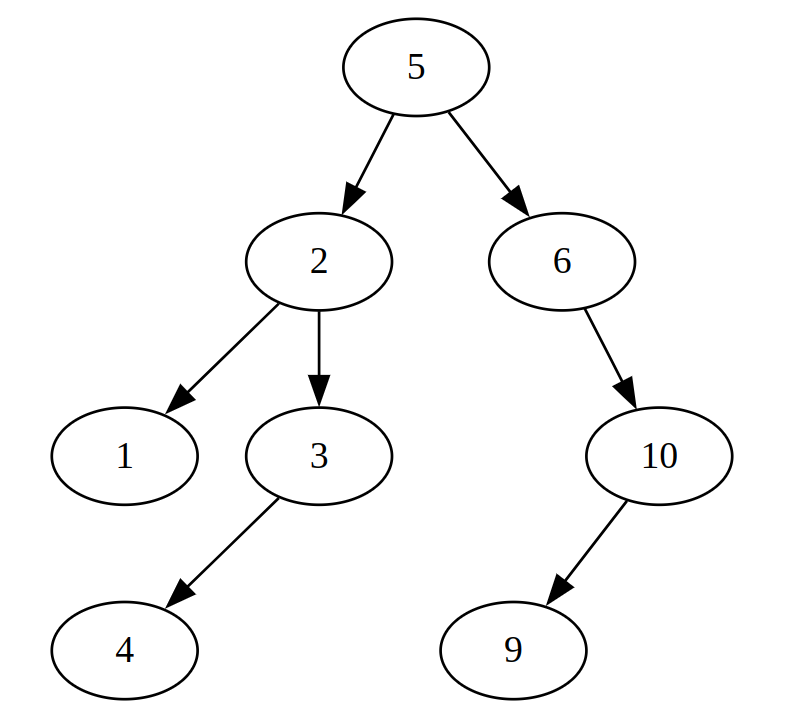
\includegraphics[width=0.35\textwidth]{figs/btree.png} % Adjust width as needed
    \caption{Árvore binária} % Will appear as "Figura 1"
    \label{fig:btree}
    % Your content (e.g., image, diagram, etc.)
\end{figlisting}

O objetivo é analisar as chamadas e usos de funções sobre operações comuns desta estrutura de dados, tais como:
\vfill\pagebreak
\begin{enumerate}
    \item Percorrimento da árvore em ordem
    \item Uso da Busca em Profundidade, do inglês: \textit{Depth First Search} (DFS)\footnote{
        Algoritmo de exploração de grafos que percorre ramificações até o fim antes de retroceder (backtracking). Usado em árvores, grafos e labirintos – estudado desde o século XIX por Trémaux (\citeauthor{wiki_dfs}, \citeyear{wiki_dfs})\cite{wiki_dfs}.
    }, para obter informações, como:
    \begin{enumerate}
        \item Checar a presença de um determinado nó na árvore
        \item Listar os nós folha da árvore
        \item Percorrer determinado nó até a raiz
        \item Calcular a altura da árvore
        \item Calcular o balanceamento da árvore
    \end{enumerate}
\end{enumerate}

\subsection{Usos}
\subsubsection{Percorrimento em ordem}
Conforme mostrado no Código \ref{listing:abp}, a árvore binária é incializada com uma lista de inteiros totalmente desordenada.
Um dos usos mais comuns da Árvore Binária são os percorrimentos em:
\begin{itemize}
    \item\textbf{Pré-Ordem}
    \item\textbf{Em-Ordem}
    \item\textbf{Pós-Ordem}
\end{itemize}

O percorrimento \textbf{Em-Ordem} pode ser utilizado para percorrer todos os nós da árvore de forma que os nós mais à esquerda são visitados primeiro. Dada a natureza de inserção dos itens em uma Árvore Binária,
sabe-se que os items cujos valores sejam menores estarão à esquerda, ao passo que os maiores à direita. Desta forma, pode-se imprimir a lista totalmente ordenada conforme mostrado no Côdigo \ref{listing:abp-in-order}:

\begin{listing}[H]
    \begin{minted}[linenos,xleftmargin=2mm,tabsize=2,breaklines,autogobble,numbersep=5pt]{python}
    tree.inOrderWalk(lambda node: print(node.value, end=" "))
    # Saída: 1 2 3 4 5 6 9 10 
    \end{minted}
    \caption{Percorrimento em ordem}
    \label{listing:abp-in-order}
\end{listing}

Nota-se no código \ref{listing:abp-in-order} o nível de abstração quando aplicada a programação funcional, pois a medida que o percorrimento ocorre, cada nó encontrado chama a funçåo lambda\footnote{
    Explicar a função lambda
} passada como segundo parâmetro de \textbf{inOrderWalk}. A função então desempenha o papel de imprimir o valor do nó.
Observa-se que ao contrário de simplesmente imprimir o nó, poderia fazer-se qualquer outra operação com o mesmo, como empilhá-los para formar uma nova lista
ordenada, por exemplo.

\subsubsection{Depth First Search (DFS)}

A Busca em profundidade (\textit{Depth First Search}) é um algoritmo que também percorre os nós de uma árvore, assim como o percorrimento em ordem.
Mas diferente de percorrer em ordem, segundo \citeauthor{wiki_dfs}\cite{wiki_dfs}: A Busca em profundidade é uma busca não-informada que progride se
aprofundando tanto quanto possível a partir do primeiro nó filho. Quando a busca chega a um nó folha, retroage-se até o próximo nó e a busca e começa
novamente.
O Código \ref{listing:dfs-percorrer} mostra o percorrimento utilizando DFS.

\begin{listing}[H]
    \begin{minted}[linenos,xleftmargin=2mm,tabsize=2,breaklines,autogobble,numbersep=5pt]{python}
    tree.dfs(lambda node: print(node.value, end=" "))
    # Saída: 5 2 1 3 4 6 10 9 
    \end{minted}
    \caption{DFS: Percorrimento}
    \label{listing:dfs-percorrer}
\end{listing}

Nota-se que o resultado apresentado agora é diferente do percorrimento em ordem apresentado no Código \ref{listing:abp-in-order}.
A busca começa a partir do nó raiz e segue até o último nó folha. Evidentemente, os valores impressos não são exibidos de forma ordenada.

\subsubsection{DFS: Encontrar um nó}

A função passada como argumento para \textbf{dfs} (ao contrário das já apresentadas), espera um valor booleano de retorno.
Este valor é utilizado para controlar quando parar a busca \textbf{dfs}. Caso uma chamada à função passada a \textbf{dfs}
retorne o valor \textbf{True}, a busca é interrompida. Quando \textbf{False}, a busca procede.\linebreak
O Código \ref{listing:dfs-encontra-no-funcoes} mostra a definição de duas funções nas linhas 1 e 2 para serem
utilizadas na \textbf{dfs}:

\begin{listing}[H]
    \begin{minted}[linenos,xleftmargin=2mm,tabsize=2,breaklines,autogobble,numbersep=5pt]{python}
    def retorna_verdadeiro(node: Node): print("Nó visitado:", node); return True
    def encontre_no(node_number: int):
        def closure(node: Node): print("Nó visitado:", node); return node.value == node_number
        return closure
    \end{minted}
    \caption{DFS: Funções de busca}
    \label{listing:dfs-encontra-no-funcoes}
\end{listing}
A função \textbf{retorna\_verdadeiro} apenas exibe o nó visitado e imediatamente retorna \textbf{True}. Enquanto que \textbf{encontre\_no}
retorna uma \textit{Closure}\footnote{
    Explicar closure
}
que compara o nó atual com um valor passado como argumento. Desta forma, \textbf{encontre\_no} se utiliza de DFS para procurar um nó na árvore.\linebreak
Conforme se observa no Código \ref{listing:dfs-encontra-no-verdadeiro}, apenas o nó raiz é visitado quando se usa \textbf{retorna\_verdadeiro}. Isto se deve ao fato de que \textbf{retorna\_verdadeiro} imediatemente retorna
o valor \textbf{True}. Quando uma função retorna \textbf{True}, a \textbf{dfs} retorna o nó atual que está sendo visitado:

\begin{listing}[H]
    \begin{minted}[linenos,xleftmargin=2mm,tabsize=2,breaklines,autogobble,numbersep=5pt]{python}
    tree.dfs(retorna_verdadeiro)
    # Saída: Nó visitado: Node(5)
    # Saída: 
    # Saída: Node(5)
    \end{minted}
    \caption{DFS: retorna\_verdadeiro}
    \label{listing:dfs-encontra-no-verdadeiro}
\end{listing}

No Código \ref{listing:dfs-encontra-no-1} pode-se observar que mais nós são visitados quando se usa \textbf{encontre\_no}. Ao final, depois de percorrer
os nós $(5,2,1)$, o nó $1$ é encontrado e retornado.

\begin{listing}[H]
    \begin{minted}[linenos,xleftmargin=2mm,tabsize=2,breaklines,autogobble,numbersep=5pt]{python}
    tree.dfs(encontre_no(1))
    # Saída: Nó visitado: Node(5)
    # Saída: Nó visitado: Node(2)
    # Saída: Nó visitado: Node(1)
    # Saída: 
    # Saída: Node(1)
    \end{minted}
    \caption{DFS: encontre\_no(1)}
    \label{listing:dfs-encontra-no-1}
\end{listing}

Finalmente, quando um determinado nó não é encontrado, a árvore inteira é percorrida sem que nada seja retornado:

\begin{listing}[H]
    \begin{minted}[linenos,xleftmargin=2mm,tabsize=2,breaklines,autogobble,numbersep=5pt]{python}
    tree.dfs(encontre_no(11))
    # Saída: Nó visitado: Node(5)
    # Saída: Nó visitado: Node(2)
    # Saída: Nó visitado: Node(1)
    # Saída: Nó visitado: Node(3)
    # Saída: Nó visitado: Node(4)
    # Saída: Nó visitado: Node(6)
    # Saída: Nó visitado: Node(10)
    # Saída: Nó visitado: Node(9)
    \end{minted}
    \caption{DFS: encontre\_no(11)}
    \label{listing:dfs-encontra-no-11}
\end{listing}

\subsubsection{DFS: Encontrar nós folha}

O Código \ref{listing:dfs-encontra-folhas} demonstra como obter uma lista dos nós folha usando \textbf{dfs} a partir da árvore.
A natureza do percorrimento \textbf{dfs} é ideal para encontrar tais nós. São encontrados 3 nós de acordo com a linha 3:

\begin{listing}[H]
    \begin{minted}[linenos,xleftmargin=2mm,tabsize=2,breaklines,autogobble,numbersep=5pt]{python}
    leafs: list[Node] = []
    tree.dfs(lambda node: leafs.append(node) if node.left is None and node.right is None else False)
    leafs
    # Saída: [Node(1), Node(4), Node(9)]
    \end{minted}
    \caption{DFS: Nós folha}
    \label{listing:dfs-encontra-folhas}
\end{listing}

\subsubsection{DFS: Nó folha até a raiz}

Uma vez que se tem a lista de nós folha, pode-se utilizar o método \textbf{goToRoot} para saber quais nós estão entre a folha e a raiz.
O Código \ref{listing:dfs-folha-raiz} mostra que os nós $(4, 3, 2, 5)$ formam o caminho entre o nó $4$ (folha), e $5$ (raiz).

\begin{listing}[H]
    \begin{minted}[linenos,xleftmargin=2mm,tabsize=2,breaklines,autogobble,numbersep=5pt]{python}
    tree.goToRoot(leafs[1], lambda node: print(node))
    # Saída: Node(4)
    # Saída: Node(3)
    # Saída: Node(2)
    # Saída: Node(5)
    \end{minted}
    \caption{DFS: Folha à raiz}
    \label{listing:dfs-folha-raiz}
\end{listing}

\subsubsection{DFS: Altura da árvore}

O Código \ref{listing:dfs-altura} demonstra a utilização de composição de funções para calcular a altura da
árvore. Nas linhas 1 a 9 são definidas as funções utilitárias. Por fim, descobre-se na linha 15 que a árvore
tem altura 4.

\begin{listing}[H]
    \begin{minted}[linenos,xleftmargin=2mm,tabsize=2,breaklines,autogobble,numbersep=5pt]{python}
    def pathToRoot(node: Node, tree: BinaryTree):
        arr: list[Node] = []
        tree.goToRoot(node, lambda n: arr.append(n))
        return arr

    def node_paths(lfs: list[Node]): return [ (leaf, pathToRoot(leaf, tree)) for leaf in lfs ]
    def node_length(node: Node, path: list[Node]): return ( node, len(path) )

    tree_heights_pipe = compose_left(
        node_paths,
        lambda arr: [ node_length(node, path) for node, path in arr ],
        lambda arr: [ size for _, size in arr ],
    )

    compose(max, tree_heights_pipe)(leafs)
    # Saída: 4
    \end{minted}
    \caption{DFS: Altura da árvore}
    \label{listing:dfs-altura}
\end{listing}

\subsubsection{DFS: Balanceamento da árvore}

Por fim, tendo-se as informações de altura dos nós folha com a ajuda da função \textbf{tree\_heights\_pipe} (Código \ref{listing:dfs-altura}, linha 9),
pode-se calcular o balanceamento da árvore conoforme mostra a linha 8 do Código \ref{listing:dfs-balanceamento}:

\begin{listing}[H]
    \begin{minted}[linenos,xleftmargin=2mm,tabsize=2,breaklines,autogobble,numbersep=5pt]{python}
    min_height = compose(min, tree_heights_pipe)(leafs)
    diff_height = compose_left(
        lambda arr: tree_heights_pipe(arr),
        lambda arr: [ i - min_height for i in arr ],
        max
    )(leafs)

    print(f"A árvore está { "des" if diff_height > 1 else "" }balanceada")
    # Saída: A árvore está balanceada
    \end{minted}
    \caption{DFS: Altura da árvore}
    \label{listing:dfs-balanceamento}
\end{listing}

Fica evidente que a árvore está totalmente balanceada pois não há nós folha com diferença de altura maior que 1.

\subsection{Implementação}
Conforme visto no Código \ref{listing:abp} (linha 1), a árvore mostrada nos exemplos pertence à bilbioreca \textbf{Btree}
que exporta dois objetos: \textbf{BinaryTree} e \textbf{Node}.\linebreak
A implementação deste módulo consiste em uma estrutura de pastas com três arquivos conforme mosta a Figura \ref{fig:modulo-btree}:

\begin{figlisting}[H]
    \centering
    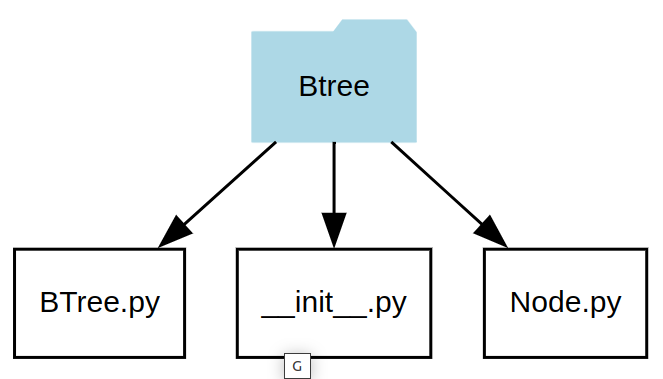
\includegraphics[width=0.35\textwidth]{figs/btree_module.png} % Adjust width as needed
    \caption{Módulo Btree} % Will appear as "Figura 1"
    \label{fig:modulo-btree}
    % Your content (e.g., image, diagram, etc.)
\end{figlisting}

\subsubsection{Node}

A árvore binária é montada com base em seus nós. Um nó é um modelo que representa um dado numérico, contento também
as referências para os nós filhos da direita e esquerda, assim como uma referência ao nó pai.\linebreak
O Código \ref{listing:impl-node} demonstra a implementação do nó:

\begin{listing}[H]
    \begin{minted}[linenos,xleftmargin=2mm,tabsize=2,breaklines,autogobble,numbersep=5pt]{python}
    from typing import Optional

    class Node:
        value: int
        parent: Optional['Node']
        right: Optional['Node']
        left: Optional['Node']

        def __init__(self, value: int):
            self.value = value
            self.left = None
            self.right = None
            self.parent = None

        def __repr__(self): return f'Node({self.value})'
    \end{minted}
    \caption{Node: Implementação}
    \label{listing:impl-node}
\end{listing}

A linha 15 define o método \textbf{\_\_repr\_\_}. Este método retorna um formato de texto que dita como
o nó deve ser exibido quando sua instância é referenciada no notebook, ou quando passada para uma função \textbf{print}.

\subsubsection{BinaryTree}

A implementação de BinaryTree é a árvore em si. No Código \ref{listing:impl-btree-ini} tem-se o método de inserção,
que consiste em inserir os nós filhos na esquerda ou direita a partir da maioridade ou menoridade com o nó pai.
\vfill
\pagebreak

\begin{listing}[H]
    \begin{minted}[linenos,xleftmargin=2mm,tabsize=2,breaklines,autogobble,numbersep=5pt]{python}
    from copy import deepcopy
    from typing import Callable
    from .Node import Node

    class BinaryTree:
        root: Node | None = None

        def __init__(self, arr: list[int]):
            for i in arr:
                self.insert(Node(i))

        def insert(self, node: Node, parent: Node | None = None):
            if self.root is None: self.root = node; return deepcopy(node)
            if parent is None: parent = self.root

            if node.value < parent.value:
                if parent.left is None:
                    node.parent = parent
                    parent.left = node
                    return deepcopy(node)
                return self.insert(node, parent.left)
            
            if parent.right is None:
                node.parent = parent
                parent.right = node
                return deepcopy(node)
            return self.insert(node, parent.right)
        ...
    \end{minted}
    \caption{BinaryTree: Implementação inicial}
    \label{listing:impl-btree-ini}
\end{listing}

\subsubsection{BinaryTree: inOrderWalk}

\begin{listing}[H]
    \begin{minted}[linenos,xleftmargin=2mm,tabsize=2,breaklines,autogobble,numbersep=5pt,firstnumber=28]{python}
    ...
        def inOrderWalk(self, callback: Callable[[Node], None] | None = None):
            def inOrderRecursive(node: Node | None):
                if node is not None:
                    inOrderRecursive(node.left)
                    if callback: callback(deepcopy(node))
                    inOrderRecursive(node.right)

            inOrderRecursive(self.root)
    ...
    \end{minted}
    \caption{BinaryTree: Método inOrderWalk}
    \label{listing:inOrderWalk}
\end{listing}

\subsubsection{BinaryTree: dfs}

\begin{listing}[H]
    \begin{minted}[linenos,xleftmargin=2mm,tabsize=2,breaklines,autogobble,numbersep=5pt,firstnumber=38]{python}
    ...
        def dfs(self, callback: Callable[[Node], bool] | None = None) -> Node | None:
            def _dfs(node: Node):
                if node is None: return
                # print(node)
                if callback:
                    res = callback(node)
                    if res:
                        return node
                if res:=_dfs(node.left): return res
                if res:=_dfs(node.right): return res

            return _dfs(self.root)
    ...
    \end{minted}
    \caption{BinaryTree: Método dfs}
    \label{listing:btree-dfs}
\end{listing}

\subsubsection{BinaryTree: goToRoot}

\begin{listing}[H]
    \begin{minted}[linenos,xleftmargin=2mm,tabsize=2,breaklines,autogobble,numbersep=5pt,firstnumber=51]{python}
    ...
        def goToRoot(self, node: Node, callback: Callable[[Node], None] | None = None):
            callback(node)
            if node == self.root: return
            self.goToRoot(node.parent, callback)
    ...
    \end{minted}
    \caption{BinaryTree: Método dfs}
    \label{listing:btree-dfs}
\end{listing}

% \begin{listing}[H]
%     \begin{minted}[linenos,xleftmargin=2mm,tabsize=2,breaklines,autogobble,numbersep=5pt]{python}
%     \end{minted}
%     \caption{AAAAAAAAAAAAA}
%     \label{listing:AAAAAAAAAAAA}
% \end{listing}
    
    % \cite{amarante2001}
    \section{REFERÊNCIAS}\\
    \bibliographystyle{plainnat}                % ou abbrvnat, unsrtnat, etc.
    \bibliography{MinhasReferencias}

    \begin{appendices}
    \clearpage
    \onecolumn
    \chapter{Apêndice A - Código Btree}
    \begin{minted}[linenos,xleftmargin=2mm,tabsize=2,breaklines,autogobble,numbersep=5pt,firstnumber=1]{python}
    from copy import deepcopy
    from typing import Callable
    from .Node import Node
    
    class BinaryTree:
        root: Node | None = None
    
        def __init__(self, arr: list[int]):
            for i in arr:
                self.insert(Node(i))
    
        def insert(self, node: Node, parent: Node | None = None):
            if self.root is None: self.root = node; return deepcopy(node)
            if parent is None: parent = self.root
    
            if node.value < parent.value:
                if parent.left is None:
                    node.parent = parent
                    parent.left = node
                    return deepcopy(node)
                return self.insert(node, parent.left)
            
            if parent.right is None:
                node.parent = parent
                parent.right = node
                return deepcopy(node)
            return self.insert(node, parent.right)
        
        def inOrderWalk(self, callback: Callable[[Node], None] | None = None):
            def inOrderRecursive(node: Node | None):
                if node is not None:
                    inOrderRecursive(node.left)
                    if callback: callback(deepcopy(node))
                    inOrderRecursive(node.right)
    
            inOrderRecursive(self.root)
    
    
        def dfs(self, callback: Callable[[Node], bool] | None = None) -> Node | None:
            def _dfs(node: Node):
                if node is None: return
                # print(node)
                if callback:
                    res = callback(node)
                    if res:
                        return node
                if res:=_dfs(node.left): return res
                if res:=_dfs(node.right): return res
    
            return _dfs(self.root)
        
        def goToRoot(self, node: Node, callback: Callable[[Node], None] | None = None):
            callback(node)
            if node == self.root: return
            self.goToRoot(node.parent, callback)
    \end{minted}
    
\end{appendices}

\end{document}
